\documentclass[12pt]{article}    % Add "draft" option for draft mode
\usepackage[paper=a4paper, top=25mm, bottom=25mm]{geometry}

% Font and encoding
\usepackage{lmodern}           % Better computer modern font
\usepackage[T1]{fontenc}       % Better glyph encoding
\usepackage[utf8]{inputenc}    % Necessary for unicode characters
\usepackage[english]{babel}    % Necessary for correct hyphenation
\usepackage{textcomp}          % Necessary to display unicode characters like €
\usepackage{csquotes}          % Quotes (\MakeOuterQuote{"} needed!)

% Other packages
\usepackage[style=authoryear]{biblatex}    % Bibliography
\usepackage[parfill]{parskip}              % Add space between paragraphs
\usepackage[hidelinks]{hyperref}           % Clickable \ref and \cite
\usepackage{graphicx}                      % Needed for figures
\usepackage{booktabs}                      % Needed for tables
\usepackage{caption}                       % Needed for captionsetup
\usepackage{subcaption}                    % Needed for subfigure and subtable
\usepackage{amsmath}                       % Better math environments and \text
\usepackage{physics}                       % e.g. for derivative formatting
\usepackage{siunitx}                       % \si{\unit} and \SI{value}{\unit}
\usepackage{titlesec}                      % Needed for titleformat
\usepackage{authblk}                       % Authors formatting

% Setup
\MakeOuterQuote{"}
% \setcounter{secnumdepth}{0}
% \titleformat{\chapter}{\normalfont\bfseries\Huge}{\thechapter}{20pt}{}
% \setlength{\parskip}{.5\baselineskip}
\setlength\parindent{0pt}
\captionsetup{width=.9\linewidth}
% \captionsetup[subfigure]{width=.9\linewidth}
\addbibresource{bib.bib}

\title{Effects of Layer Freezing when Transferring DeepSpeech from English to German}
\author[1]{\textbf{Onno Eberhard}}
\author[ ]{\textbf{Torsten Zesch}}
\affil[ ]{Language Technology Lab}
\affil[ ]{University of Duisburg-Essen}
\affil[1]{\href{mailto:onno.eberhard@stud.uni-due.de}{\texttt{onno.eberhard@stud.uni-due.de}}}
\date{}

\begin{document}
\maketitle

\begin{abstract}\noindent
In this paper, we train Mozilla's DeepSpeech architecture on a German language speech dataset and compare the results of different training methods. We build on previous efforts by \textcite{agarwal-zesch-2019-german} and reproduce their results by training the model from scratch. We improve upon these results by using an English pretrained version of DeepSpeech for weight initialization and experiment with the effects of freezing different layers during training. We see that freezing even one layer already improves the results dramatically.
\end{abstract}

\section{Introduction}
The field of automatic speech recognition is dominated by research specific to the English language. There exist plenty available text-to-speech models pretrained on (and optimized for) English data. When it comes to German, the range of available pretrained models becomes much sparser. In this paper, we train Mozilla's implementation\footnote{\url{https://github.com/mozilla/DeepSpeech}} of Baidu's DeepSpeech architecture \parencite{hannun2014deep} on German speech data. We use transfer learning to leverage the availability of a pretrained English version of DeepSpeech and observe the difference made by freezing different layers during training. The rationale for using transfer learning is not only that English and German are closely related languages. In fact, one could argue that they are very different in this context, because DeepSpeech is trained to directly infer written characters from audio data and English and German pronunciations of some characters differ greatly. However, the first few layers of the DeepSpeech network are likely not inferring the final output character, but rather lower lever features of the spoken input, such as phonemes, which are shared across different languages. Thus, this approach should also work for languages which are not related at all. It is to be expected that the model should give better results when trained on a small dataset than a model trained from scratch, because it does not have to learn these lower level features again.

\section{Training}
\subsection{DeepSpeech architecture}
Mozilla's DeepSpeech implementation differs in many ways from the original model presented by \textcite{hannun2014deep}. The architecture is described in detail in the official documentation\footnote{\url{https://deepspeech.readthedocs.io/en/latest/DeepSpeech.html}} and is depicted in Figure \ref{fig:ds}. From the raw speech data, Mel-Frequency Cepstral Coefficients \parencite{imai1983cepstral} are extracted and passed to a 6-layer deep recurrent neural network. The first three layers are fully connected with a ReLU activation function. The fourth layer is a Long Short-Term Memory unit \parencite{hochreiter1997long}; the fifth layer is again fully connected and ReLU activated. The last layer outputs probabilities for each character in the language's alphabet. It is fully connected and uses a softmax activation for normalization. The character-probabilities are used to calculate a Connectionist Temporal Classification (CTC) loss function \parencite{graves2006connectionist}. The weights of the model are optimized using the Adam method \parencite{kingma2014adam} with respect to the CTC loss.

\begin{figure}[ht]
    \centering
    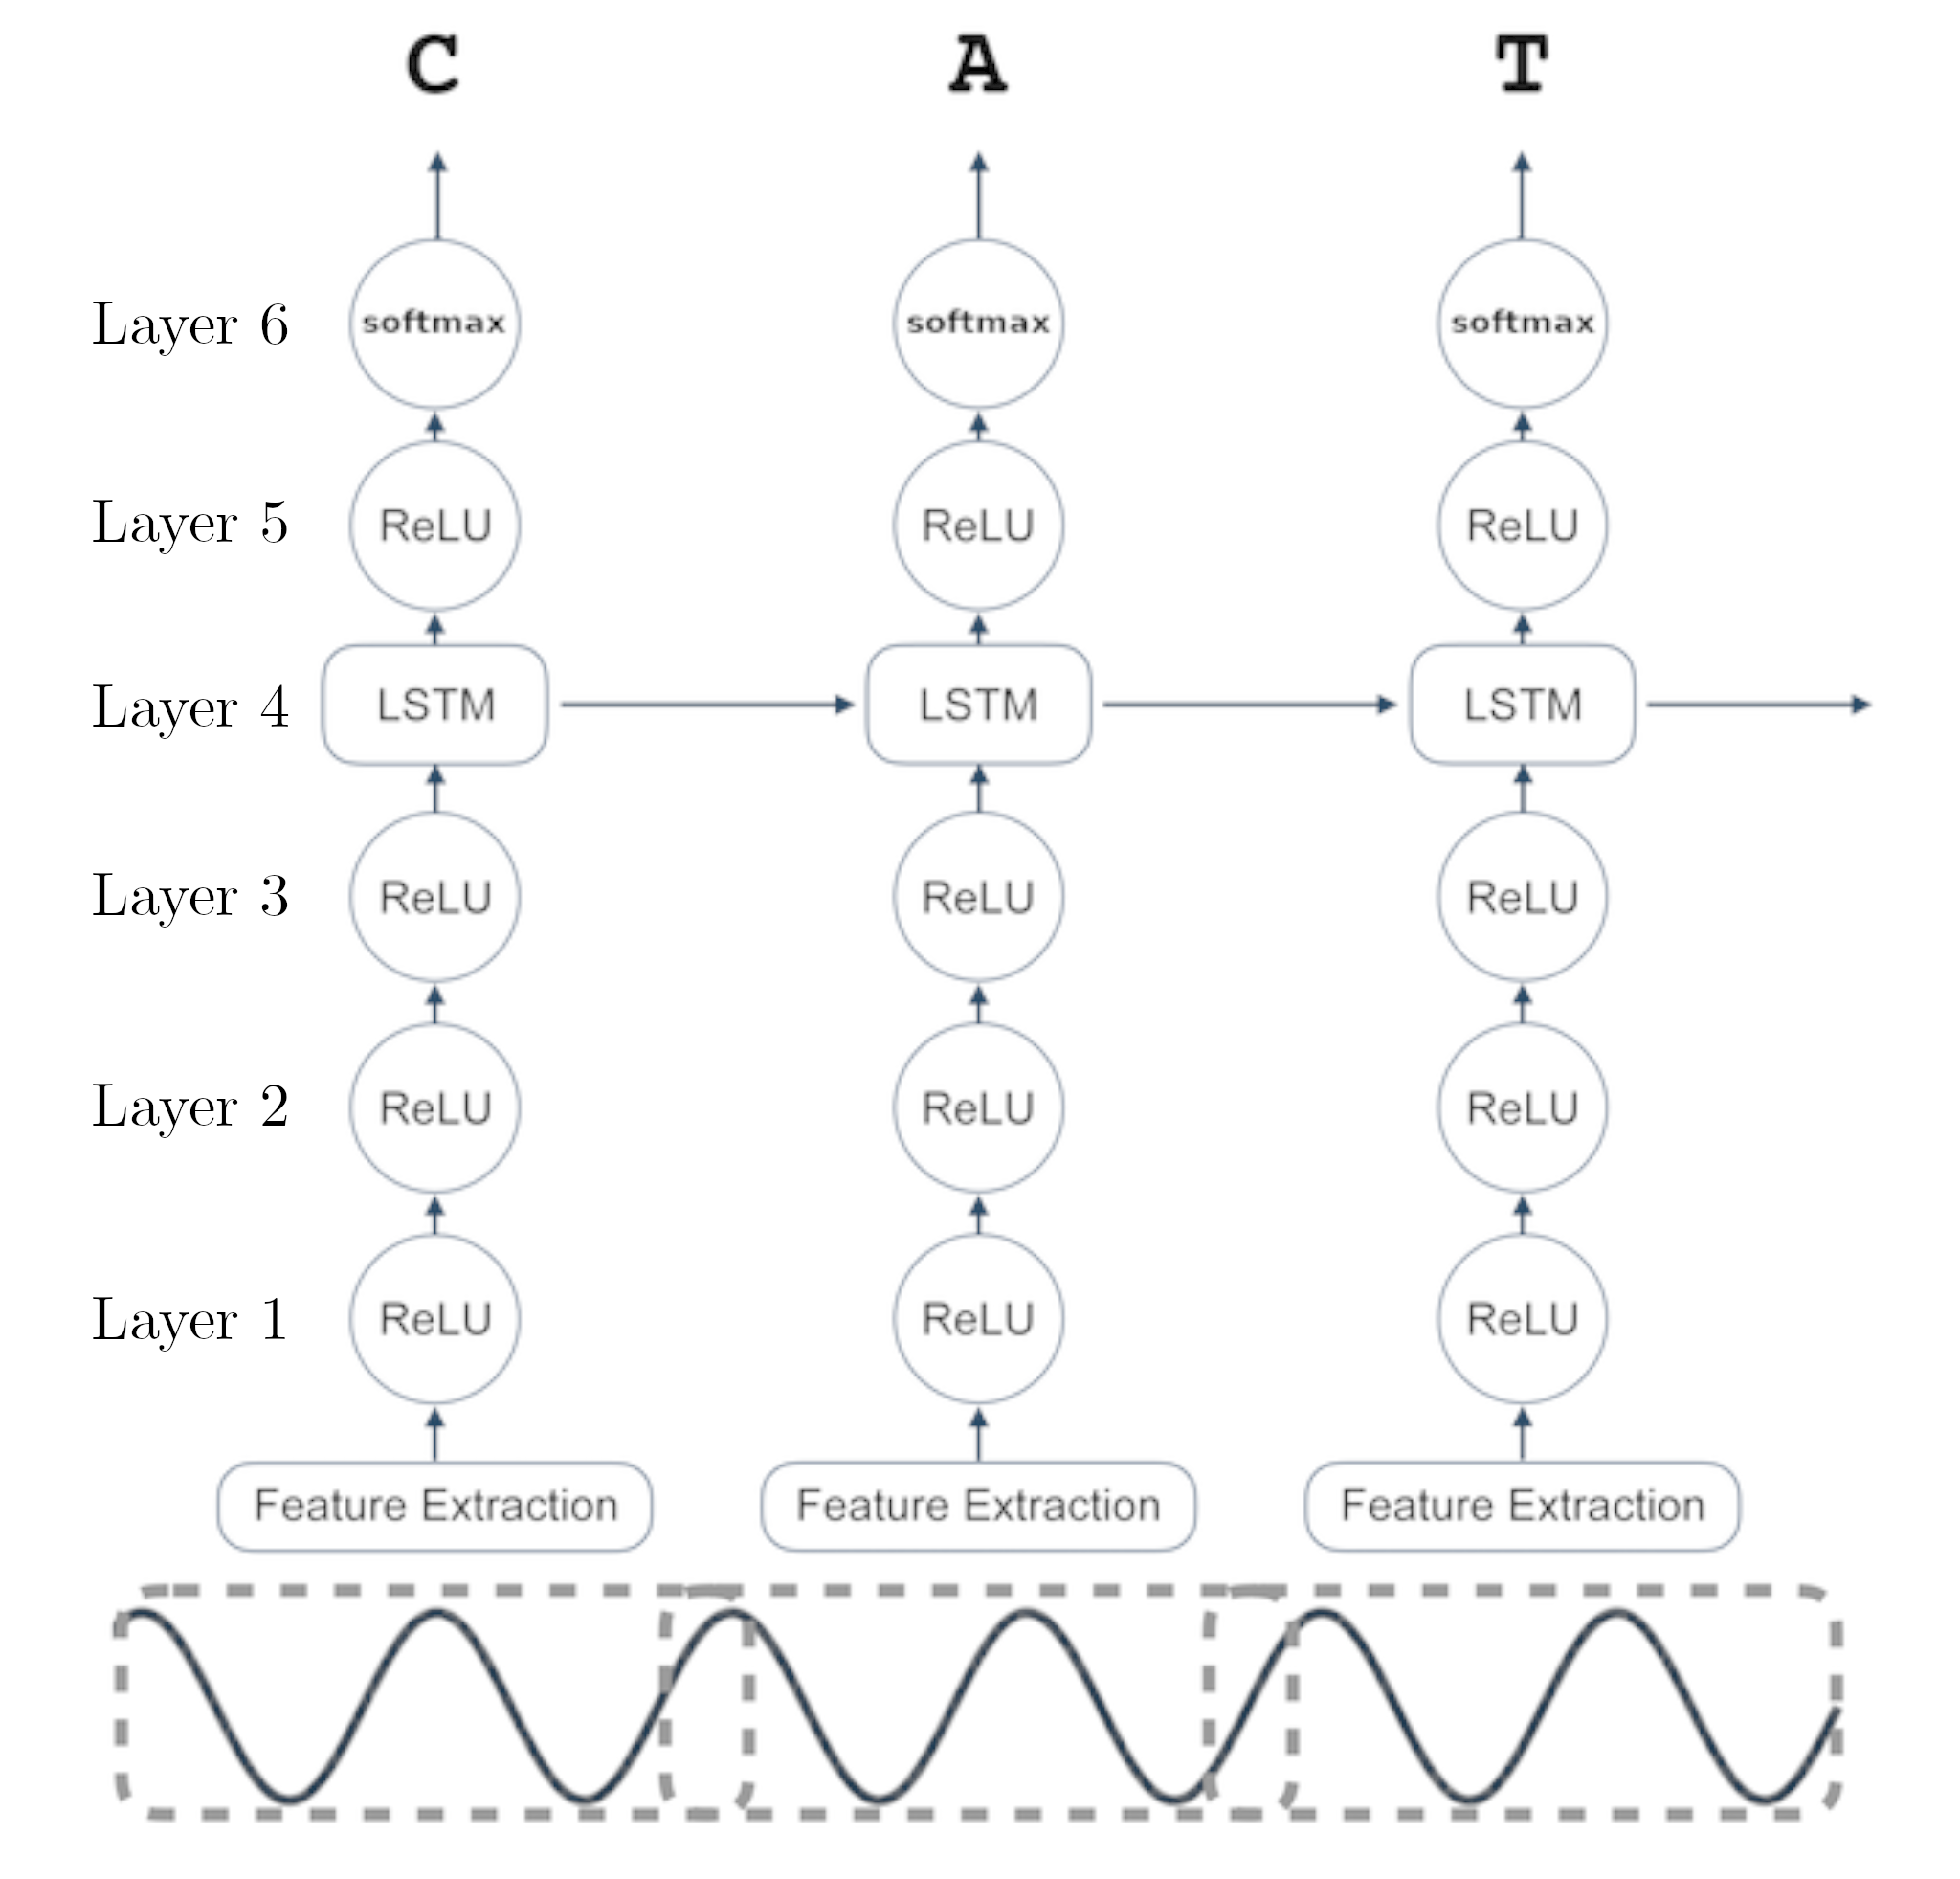
\includegraphics[width=.85\textwidth]{ds.png}
    \caption{DeepSpeech architecture (adapted from the official documentation\protect\footnotemark[\value{footnote}])}
    \label{fig:ds}
\end{figure}

\subsection{Training Details} \label{sec:training}
In transfer learning, all weights of the model are initialized to those of the English pretrained model, which is provided by Mozilla\footnote{\url{https://github.com/mozilla/DeepSpeech/releases}}. In addition to transfer learning, we also train the model from scratch with random weight initialization, thereby reproducing a result from \textcite{agarwal-zesch-2019-german}.

In total, we train 6 different models:
\begin{enumerate}
    \item The whole model from scratch ("Complete Training")
    \item The model with weights initialized to those of the English pretrained model, all weights are optimized during training ("Simple Transfer")
    \item The English-initialized model with the first layer frozen
    \item The English-initialized model with the first two layers frozen
    \item The English-initialized model with the first three layers frozen
    \item The English-initialized model with the first three and the fifth layer frozen
\end{enumerate}

We used Mozilla's DeepSpeech version 0.7.4 for training the model from scratch and version 0.7.3 for the transfer learning approach. The complete training script is available online\footnote{\url{https://github.com/onnoeberhard/deepspeech-paper/blob/master/training.sh}}. The modified versions of DeepSpeech that utilize layer freezing are also available online\footnote{\url{https://github.com/onnoeberhard/deepspeech-transfer}, the different versions with a different number of frozen layers are in the branches \emph{transfer-1}, \emph{\mbox{transfer-2}}, \emph{transfer} and \emph{\mbox{transfer-4}}.}. The weights were frozen by adding \texttt{trainable=False} at the appropriate places in the TensorFlow code. For all models, we had to reinitialize the last layer, because of the different alphabet sizes of German and English (ä, ö, ü).

We trained the models on the German-language Mozilla Common Voice 2.0 speech dataset\footnote{\url{https://voice.mozilla.org/en/datasets}}. For inference and testing we used the language model KenLM \parencite{heafield-2011-kenlm}, trained on the corpus described in \parencite[Section~3.2]{Radeck-Arneth2015}. The text corpus consists of a mixture of text from the sources Wikipedia and Europarl as well as crawled sentences. The whole corpus was preprocessed with MaryTTS \parencite{schroder2003german} and cleaned in the same way as described in \textcite{agarwal-zesch-2019-german}. All these steps were chosen to be identical to those taken by \textcite{agarwal-zesch-2019-german}, such that comparison of results would be as meaningful as possible.

In training each model, we used a batch size of 24, a learning rate of 0.0005 and a dropout rate of 0.4. We did not perform any hyperparameter optimization. These hyperparameters, as well as those selected for training the language model, differ from those chosen by \textcite{agarwal-zesch-2019-german}. This explains why our results differ even though the same model and training data was used. The training was done on a Linux machine with 96 Intel Xeon Platinum 8160 CPUs @ 2.10GHz, 256GB of memory and an NVIDIA GeForce GTX 1080 Ti GPU with 11GB of memory. Training the models for 30 epochs took approximately one hour per model.

\section{Results}
The test results from the six different models described in section \ref{sec:training} are compiled in table \ref{tab:results}. For testing, the epoch with the best validation loss during training was taken for each model. The last row is taken from \textcite[Table~3]{agarwal-zesch-2019-german} and describes only the result of training with the same data as we did. The difference between our result without transfer learning (WER 0.697) and theirs (WER 0.797) likely stems from the difference in hyperparameters used. Figures \ref{fig:3c} and \ref{fig:4c} show the learning curves for all training procedures, with the green line (3 frozen layers) being the same in both plots. The epochs used for testing are also marked in the figures.

\begin{table}[ht]
    \centering
    \vspace{5mm}
    \begin{tabular}{lrrr}
        \toprule
        Method & WER \\
        \midrule
        Complete Training & 0.697 \\
        Simple Transfer & 0.627 \\
        1 Frozen Layer & 0.483 \\
        2 Frozen Layers & 0.443 \\
        \textbf{3 Frozen Layers} & \textbf{0.437} \\
        4 Frozen Layers & 0.462 \\
        \cite{agarwal-zesch-2019-german} & 0.797 \\
        \bottomrule
    \end{tabular}
    \caption{Testing results (Word Error Rate)}
    \label{tab:results}
\end{table}

\begin{figure}[ht]
    \centering
    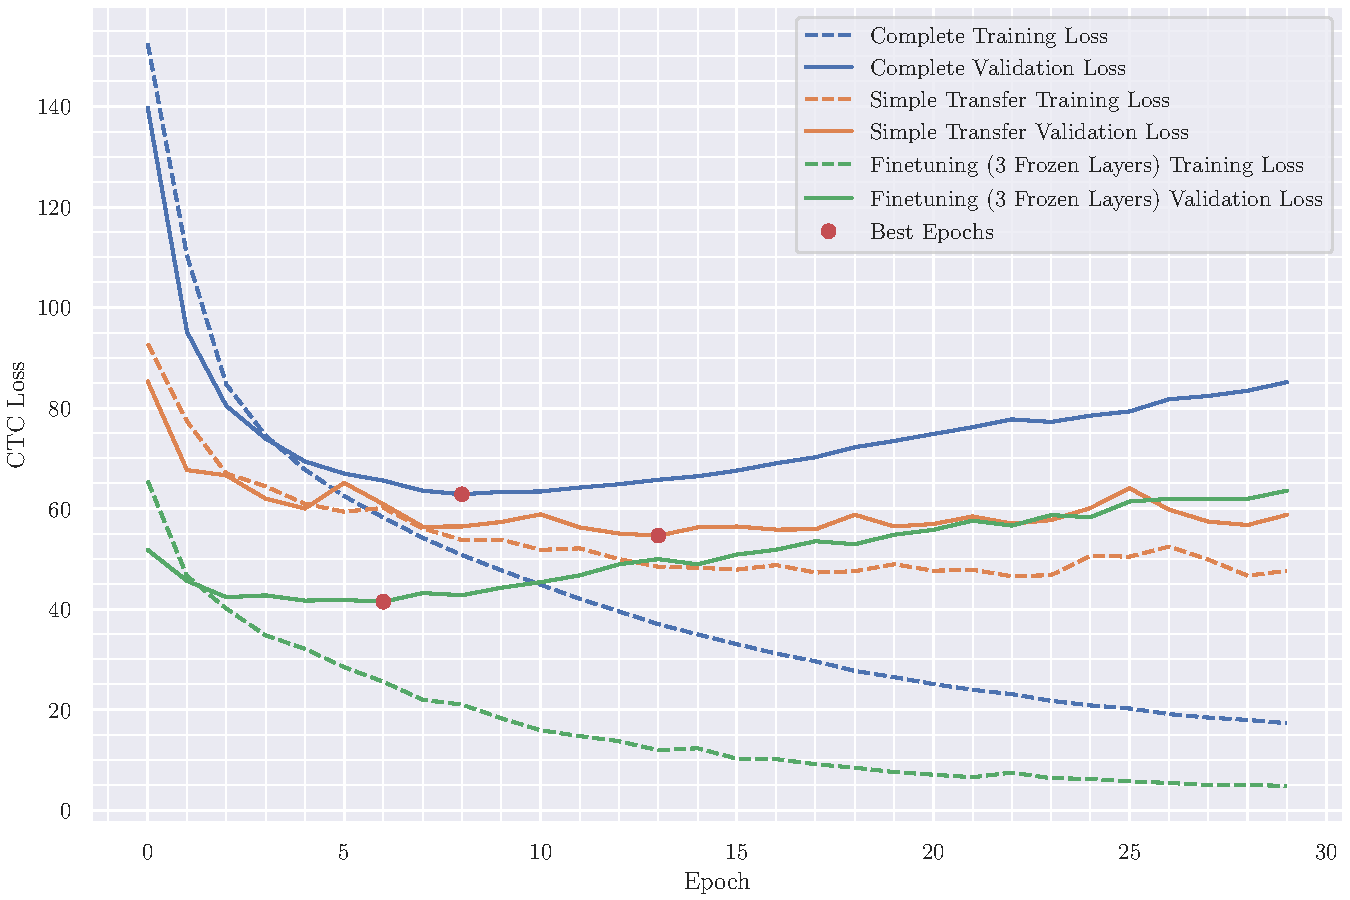
\includegraphics[width=\textwidth]{../3curves.pdf}
    \caption{Learning curves: With and without transfer learning and layer freezing}
    \label{fig:3c}
\end{figure}

\begin{figure}[ht]
    \centering
    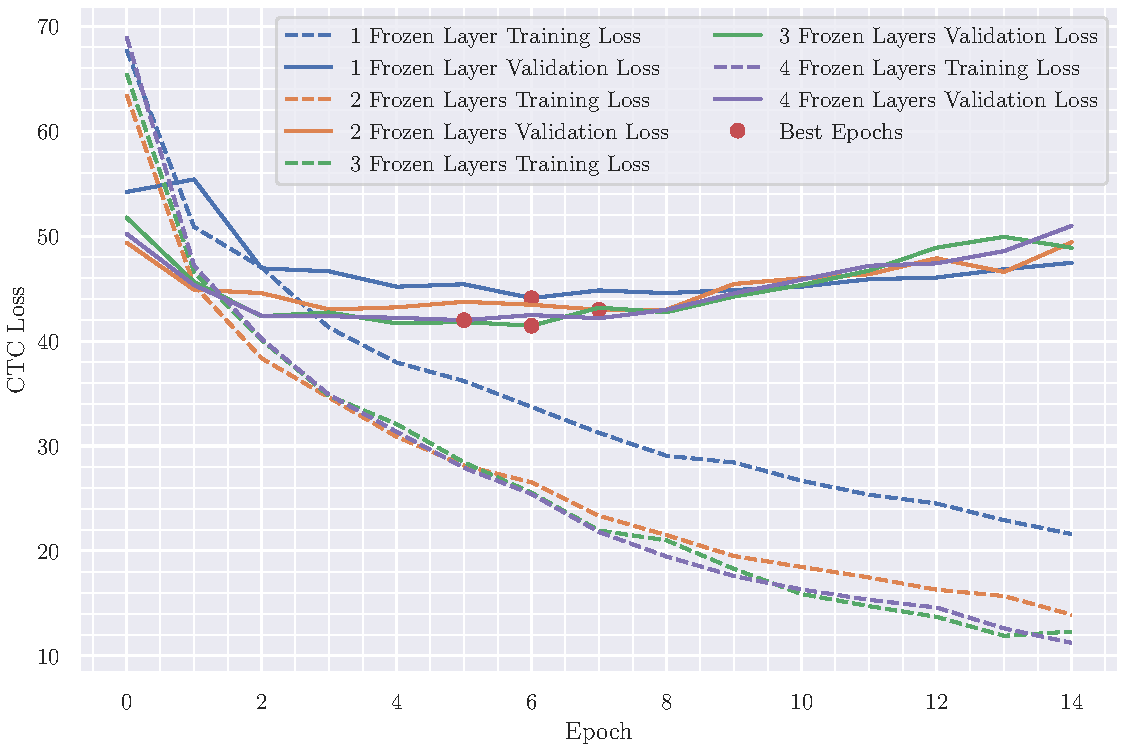
\includegraphics[width=\textwidth]{../4curves.pdf}
    \caption{Learning curves: Comparison of freezing a different number of layers}
    \label{fig:4c}
\end{figure}

The best results were achieved by the model with the first three layers frozen during training. It is notable however, that the other three models that utilize layer freezing are not far off. The training curves look remarkably similar (see Figure~\ref{fig:4c}). All four models achieve much better results than the two models without layer freezing. The results seem to indicate that freezing the first layer brings the largest advantage in training, with diminishing returns on freezing the second and third layers. Additionally freezing the fifth layer slightly worsens the result.

The model with four frozen layers could only optimize the LSTM weights and the weights of the output layer. It is surprising that it still achieves good results. It might be interesting to see what happens when the LSTM layer is frozen. It is probable that with a larger dataset the benefits of freezing weights decrease and better results are achieved with freezing fewer or no layers. However, for languages or dialects with little available training data this transfer learning approach seems promising.

A next step might be to train these models with more training data and see if layer freezing is still beneficial. The chosen speech dataset (Mozilla Common Voice 2.0) is not very large; \textcite{agarwal-zesch-2019-german} achieved a best result of 0.151 WER when training the model on a large dataset, in contrast to a result of 0.797 WER when training the same model on only the dataset used here.

The TensorFlow checkpoint for our best model (3 frozen layers) is available online\footnote{\url{https://onnoeberhard.com/deepspeech}}.

\section{Further Research}
An interesting idea for further research is to use a different pretrained model than the English one. English seems to work alright for transferring to German, but it is possible that the lower level language features extracted by a model only trained for recognizing English speech are not sufficient for transferring to certain other languages. For example, when just transcribing speech there is no need for such a model to learn intonation features. This might be a problem when trying to transfer such a pretrained model to a tonal language like Mandarin or Thai. There might also be phonemes that don't exist or are very rare in English but abundant in other languages. 

For these reasons one could try and build a new model that is trained on language data from many different languages, with the same task of transcribing speech to text. The model will not be good at this task, because it would have to learn all these languages at the same time and differentiate between them, which is not easy without a very large number of tunable parameters\footnote{A GPT-3-sized \parencite{brown2020language} model might be able to learn many languages simultaneously}. However, if trained correctly, it should at least extract the lower level features from these languages. This means that it should be possible to transfer this "bad" model to any language and get good results without large amounts of training data, when using layer freezing again. One might want to make the initial "bad" model much larger than DeepSpeech because it can be trained on large amounts of speech data from many languages. The size does not matter too much when transferring, because most of the weights would be frozen.

To implement this idea, the DeepSpeech implementation used in this paper is not sufficient, because it does not support training on languages with different alphabet sizes at the same time. Instead, it might be possible to use a multitask learning approach, where the model is not only trained to output the correct character, but also the language of the current utterance. The predicted language can then be used to select the correct alphabet used for predicting the current character.

\section{Summary}
Transfer learning seems to be a powerful approach to train an automatic speech recognition system on a small dataset. The effect we saw when transferring DeepSpeech from English to German was not very large when just initializing the parameters, but only freezing the first layer already improved the results dramatically. Freezing more layers improved the outcome even more, but with larger training datasets this might have adverse effects.

\section{Acknowledgements}
We want to thank Aashish Agarwal for valuable help in setting up DeepSpeech and for providing preprocessing scripts as well as the hyperparameters we used for training.

\printbibliography

\end{document}
